\documentclass[a4paper, 12pt]{article}
\usepackage[T2A,T1]{fontenc}
\usepackage[utf8]{inputenc}
\usepackage[english, russian]{babel}
\usepackage{graphicx}
\usepackage[hcentering, bindingoffset = 10mm, right = 15 mm, left = 15 mm, top=20mm, bottom = 20 mm]{geometry}
\usepackage{multirow}
\usepackage{lipsum}
\usepackage{amsmath, amstext}
\usepackage{siunitx}
\usepackage{subcaption}
\usepackage{wrapfig}
\usepackage{mathrsfs}
\usepackage{adjustbox}
\usepackage{enumerate, indentfirst, float}
\usepackage{capt-of, svg}
\usepackage{icomma}
\usepackage{xcolor}

\newenvironment{bottompar}{\par\vspace*{\fill}}{\clearpage}
 
\begin{document}
\begin{titlepage}

\newcommand{\HRule}{\rule{\linewidth}{0.5mm}} % Defines a new command for the horizontal lines, change thickness here

\center % Center everything on the page
 
%----------------------------------------------------------------------------------------
%	HEADING SECTIONS
%----------------------------------------------------------------------------------------

\textsc{\LARGE Московский \\[0.5cm] Физико-Технический Институт}\\[1,5cm] % Name of your university/college
\textsc{\Large Кафедра общей физики}\\[0.5cm] % Major heading such as course name
\textsc{\large Лабораторная работа \textnumero  3.3.4}\\[0.5cm] % Minor heading such as course title

%----------------------------------------------------------------------------------------
%	TITLE SECTION
%----------------------------------------------------------------------------------------

\HRule
\\[0.4cm]
{ \huge \bfseries Эффект Холла в полупроводниках}
\\[0.2cm] % Title of your document
\HRule
\\[1.5cm]


 
%----------------------------------------------------------------------------------------
%	AUTHOR SECTION
%----------------------------------------------------------------------------------------


	\begin{flushleft} \large
	\emph{Студент:}\\
	Павел \textsc{Северилов} \\
	671 группа
	\end{flushleft}



\begin{bottompar}
	\begin{center}
		
\includegraphics[width = 80 mm]{logo.jpg}
	\end{center}
	{\large \today}

\end{bottompar}
\vfill % Fill the rest of the page with whitespace

\end{titlepage}

\section{Цель работы}
Измерение подвижности и концентрации носителей заряда в полупроводниках.

В работе используются: \textit{электромагнит с источником питания, амперметр, миллиамперметр, милливеберметр, реостат, цифровой вольтметр, источник питания, образцы легированного германия.}


\subsection*{Теоретическая часть}

\subsubsection*{Дырки}

Эффект Холла, возникающий в проводниках, происходит из-за наличия некоторого количества свободных электронов в зоне проводимости и такого же количества дырок в валентной зоне. Чтобы понять причину образования дырок, нужно рассмотреть дырочную проводимость.


Дырочную проводимость можно объяснить при помощи следующей аналогии: если представить ряд людей, сидящих в аудитории, где нет запасных стульев. Когда кто-нибудь из середины ряда хочет уйти, он      перелезает через спинку стула в пустой ряд и уходит. Здесь пустой ряд — аналог зоны проводимости, а ушедшего человека можно сравнить со свободным электроном.
Теперь представим, что ещё кто-то пришёл и хочет сесть. Из пустого ряда плохо видно, поэтому там он не садится. Вместо этого человек, сидящий возле свободного стула, пересаживается на него, вслед за ним это повторяют и все его соседи. Таким образом, пустое место как бы двигается к краю ряда. Когда это место окажется рядом с новым зрителем, он сможет сесть.
В этом процессе каждый сидящий передвинулся вдоль ряда. Если бы зрители обладали отрицательным зарядом, такое движение было бы  \textit{электрической проводимостью}. Если вдобавок стулья заряжены положительно, то ненулевым суммарным зарядом будет обладать только свободное место. Однако на самом деле, из-за свойств кристаллической решётки, дырка не локализована в определённом месте, как описано выше, а размазана по всему полупроводнику.

\subsubsection*{Эффект Холла}

Магнитного поле в проводнике действует на свободные электроны в зоне проводимости, поэтому между гранями наблюдается добавочная разность потенциалов, связанная с силой Лоренца. 

$$\boldsymbol{F_\text{Л}}  = -e \boldsymbol{E} - e \langle \boldsymbol{\upsilon} \rangle \times \boldsymbol{B},$$
где $e$ - абсолютная величина заряда электрона, $\boldsymbol{B}$ - индукция магнитного поля, $\boldsymbol{E}$ - напряженность электрического поля, $ \langle \upsilon \rangle$ - средняя скорость заряда.

Из этого выражения получим разность потенциалов между двумя гранями:

\begin{equation}
U = -E_zl = - | \langle \upsilon \rangle | B l
\label{eq:pot_dif}
\end{equation}
С этой возникшей разностью потенциалов и связан Эффект Холла.
Далее, если выразить ток:
$$ I = ne |\langle \upsilon \rangle |  l a$$
И совместить его с \ref{eq:pot_dif}, получим ЭДС Холла:

\begin{equation}
\mathscr{E}_x = U = - \dfrac{IB}{nea} = -R_x \cdot \dfrac{IB}{a},
\label{eq: Hall}
\end{equation}

где $R_x = \dfrac{1}{ne}$ называется \textit{постоянной Холла.}

\subsection*{Установка и параметры измерения}

\begin{wrapfigure}[15]{l}{0.7 \textwidth}
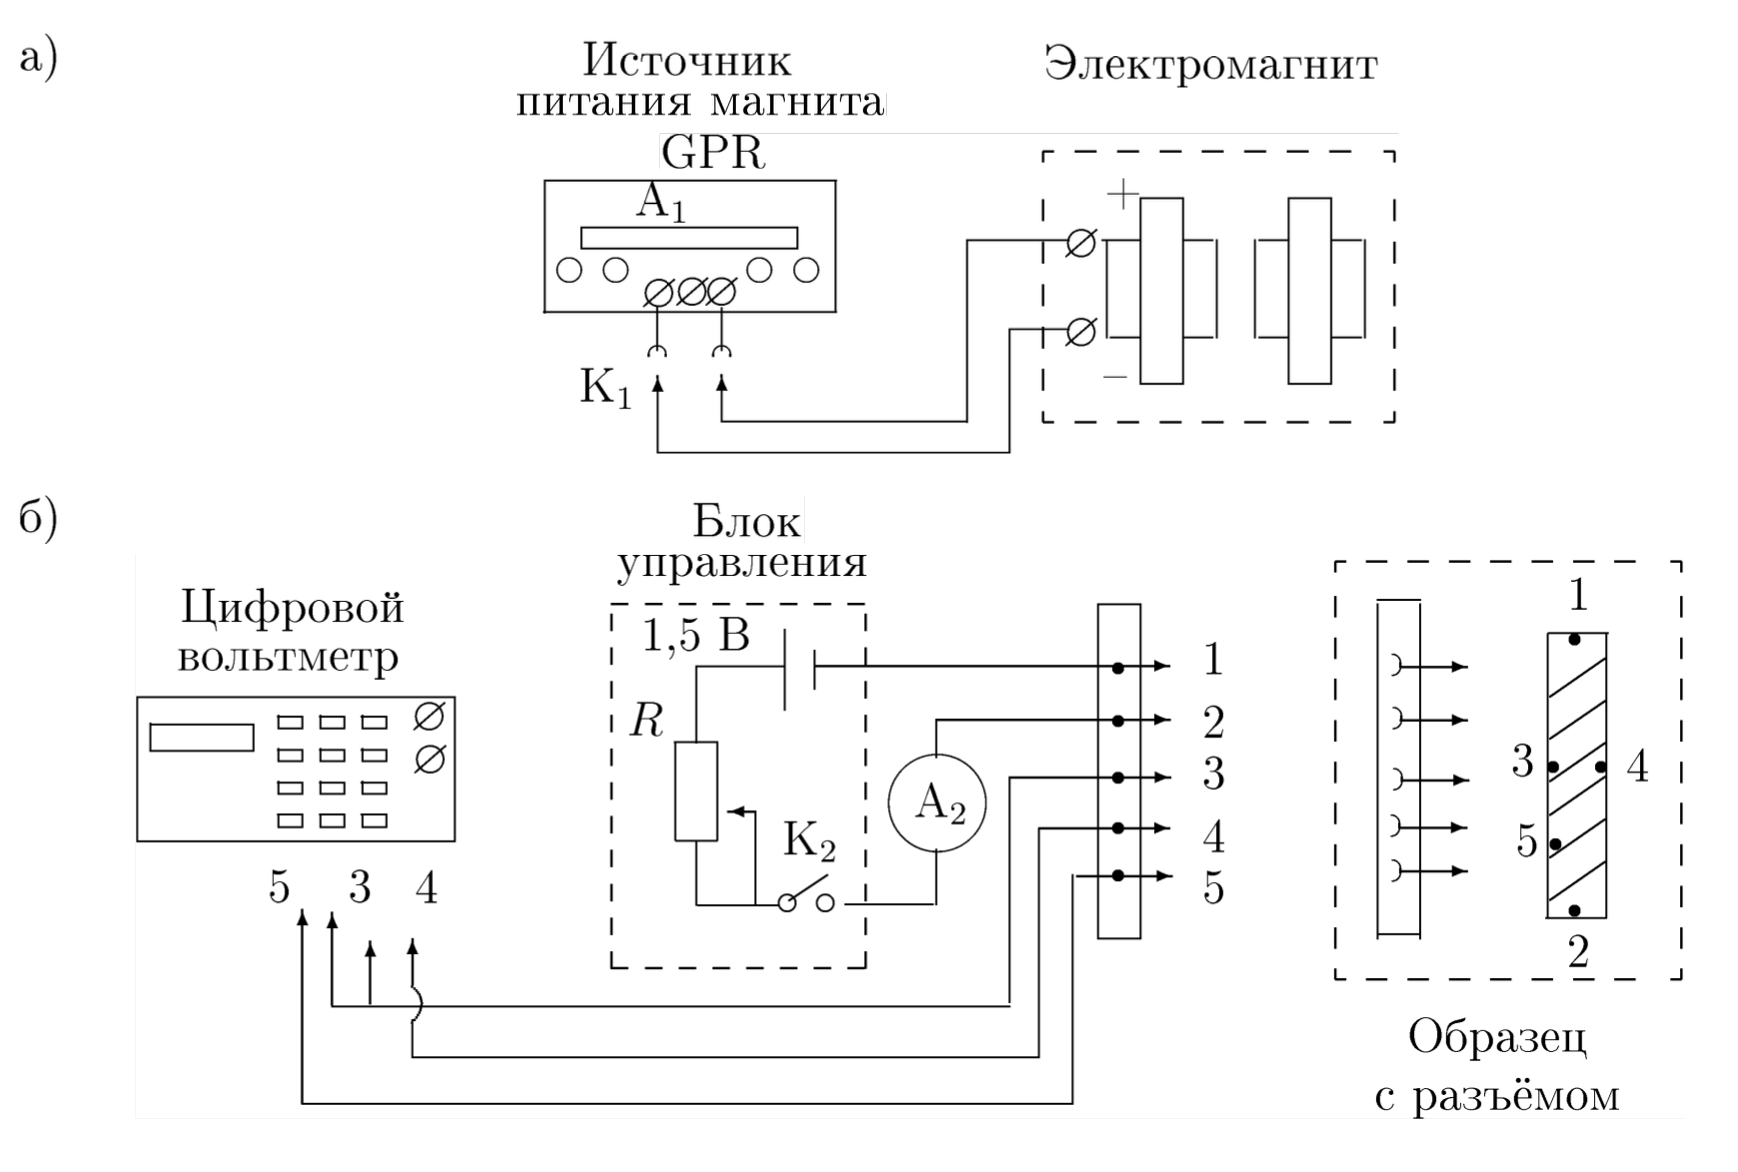
\includegraphics[width = 0.7 \textwidth]{Scheme1}
			\caption{Схема установки для измерения эффекта Холла в полупроводниках}
\end{wrapfigure} 

		$$\text{Параметры установки:}$$
$$a = 2.2 \text{ мм}$$
$$L_{35} = 3 \text{ мм}$$
$$l = 2.5 \text{ мм}$$
\vspace{5 cm}

В нашей установке вдоль длинной стороны образца будет течь ток, величина которого регулируется реостатом $R_2$. Так как он помещен в электромагнит, между точками \textit{3 и 4} будет возникать разность потенциалов $U_{34}$, которую мы будем измерять. 

Однако между точками \textit{3 и 4} будет возникать некоторое дополнительное падение напряжения $U_{0}$, так как эти точки оказываются не на одной эквипотенциали. Исключить это влияние можно с помощью изменения направления магнитного поля: в одном случае $U_{34} = U_{0} - \mathscr{E}_x $, в другом  $U_{34} = U_0 - \mathscr{E}_x $. Тогда с помощью полуразности избавимся от $U_{0}$ в наших измерениях. 

\section{Работа и измерения}
Параметры установки:
$a = 1,5 \text{ мм}$; 
$L_{35} = 3,0 \text{ мм}$;
$l = 1,7 \text{ мм}$
\subsection*{Калибровка установки}

Прокалибруем электромагнит -- определим связь между индукцией B магнитного поля в зазоре электромагнита и током $I_m$ через обмотку магнита. (с учетом $\text{Ф} = BSN$, $SN = 75$ $\text{см}^2$ вит)


\begin{table}[H]
\centering
\begin{tabular}{|c|c|c|c|c|c|c|c|c|c|}
\hline
$\text{Ф, мВб}$&-1.2&-1.7&-2.2&-2.8&-3.3&-3.8&-4.4&-4.8&-5.2\\ \hline
$I_m, \text{ А}$ & 0.20    & 0.30   & 0.40 & 0.50   & 0.60   & 0.70     & 0.80    &0.90  & 1.00 \\ \hline
$B, \text{ Тл}$ & 0,16&0,2267&0,2933&0,3733&0,44&0,5067&0,5867&0,64&0,693\\ \hline
\end{tabular}
\caption{Данные для калибровки установки}
\end{table}

Построим по полученным данным график.

	\begin {figure}[H]
		\begin{center}
			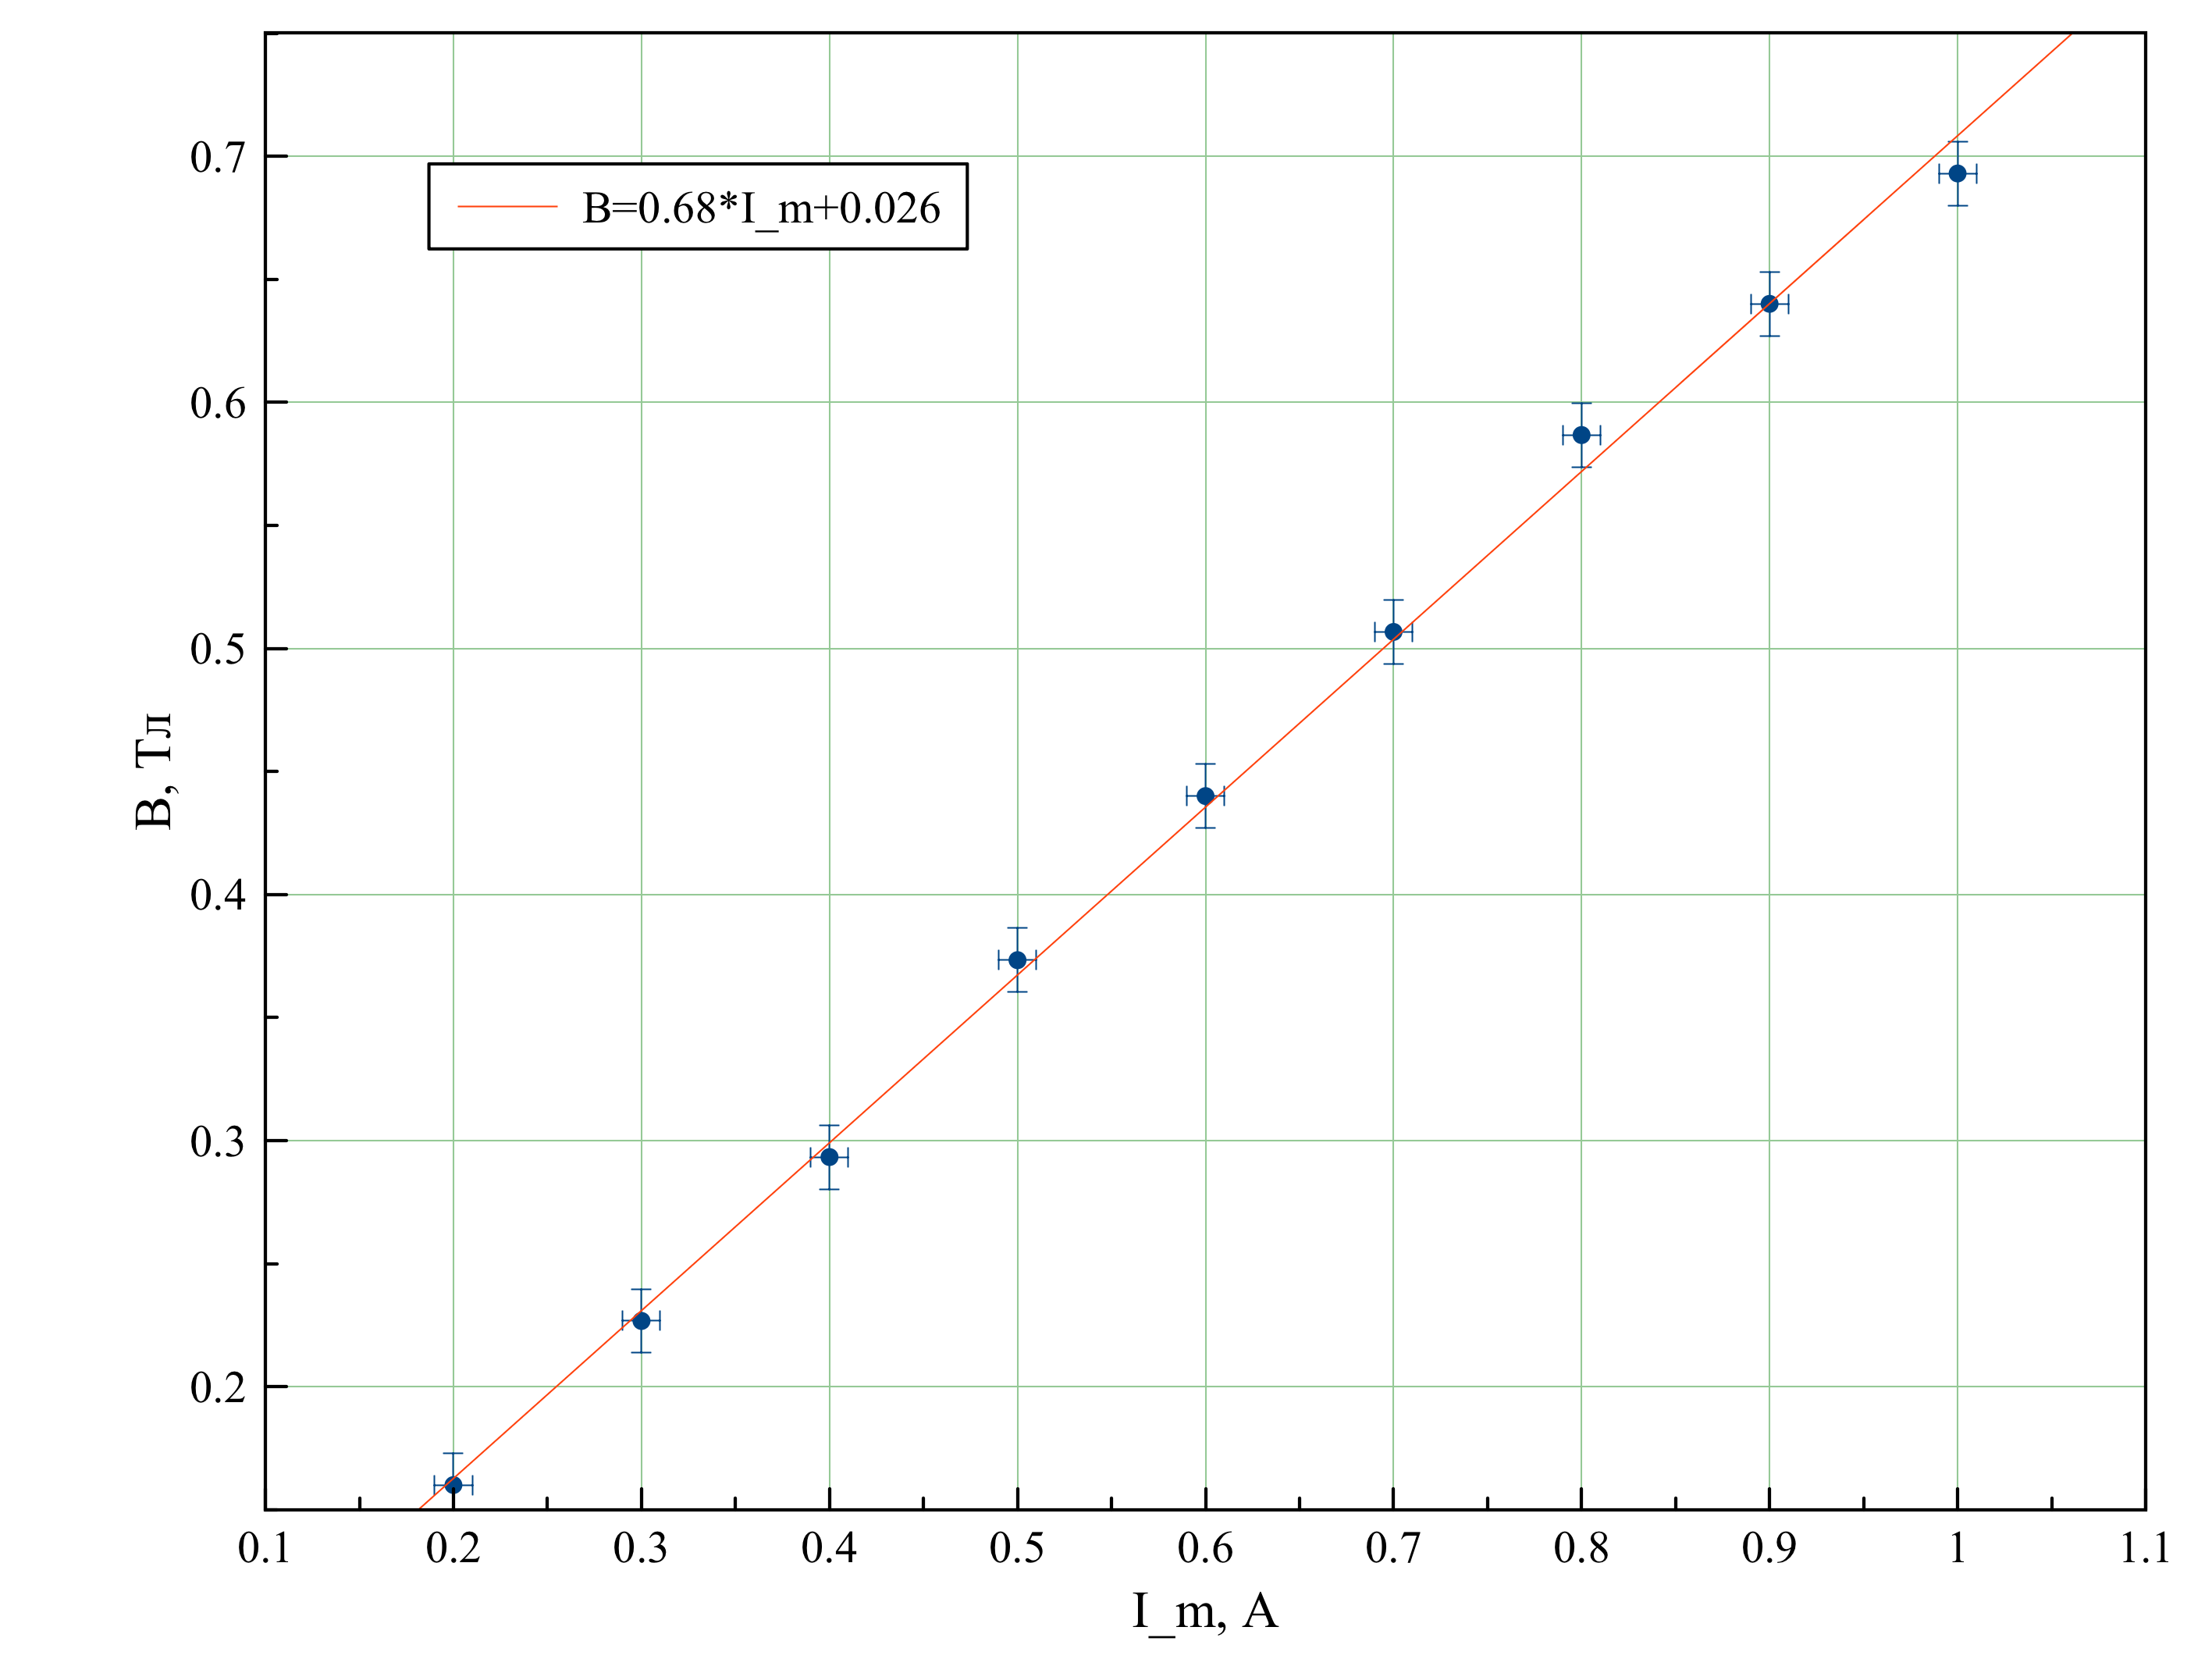
\includegraphics[width = 0.9 \textwidth]{B(I)}
			\caption{Уравнение для калибровки установки}
		\end{center}
	\end {figure}
	
Проведем измерение ЭДС Холла при разных значениях тока через образец. 

\begin{table}[H]
\centering
\resizebox{\textwidth}{!}{%
\begin{tabular}{|c|c|c|c|c|c|c|c|c|c|c|}
\hline
$U_0,  \text{мВ}$	& $I_{34},  \text{мА}$	& $I_m, A$	& 0,3	& 0,4& 	0,5& 	0,6& 	0,7& 	0,9& 	1 \\ \hline
-& 	-& 	$B,  \text{Тл}$	& 0,23& 	0,298& 	0,366& 	0,434& 	0,502& 	0,638& 	0,706 \\ \hline
0,005& 	0,3& $	U_{34},  \text{мВ}$& 	0,04& 	0,052& 	0,065& 	0,075& 	0,085& 	0,105& 	0,114 \\ \hline
-& 	-& 	$\mathscr{E}_x, \text{мВ}$	& 0,045& 	0,057& 	0,07& 	0,08& 	0,09& 	0,11& 	0,119 \\ \hline
0,006& 	0,4& $	U_{34},  \text{мВ}$& 	0,05& 	0,066& 	0,082& 	0,098& 	0,111& 	0,138& 	0,151 \\ \hline
-& 	-& 	$\mathscr{E}_x, \text{мВ}$& 	0,056& 	0,072& 	0,088& 	0,104& 	0,117& 	0,144& 	0,157 \\ \hline
0,006& 	0,5	&$	U_{34},  \text{мВ}$& 	0,062& 	0,082& 	0,1& 0,12& 	0,138& 	0,171& 	0,187 \\ \hline
-& 	-& 	$\mathscr{E}_x, \text{мВ}$& 	0,068& 	0,088& 	0,106& 	0,126& 	0,144& 	0,177& 	0,193 \\ \hline
0,003& 	0,7	& $	U_{34},  \text{мВ}$& 	0,081& 	0,109& 	0,137& 	0,163& 	0,187& 	0,235& 	0,256 \\ \hline
-& 	-& 	$\mathscr{E}_x, \text{мВ}$& 	0,084& 	0,112& 	0,14& 	0,166& 	0,19& 	0,238& 	0,259 \\ \hline
0,002& 	0,9& 	$	U_{34},  \text{мВ}$& 	0,103& 	0,137& 	0,171& 	0,204& 	0,238& 	0,299& 	0,324 \\ \hline
-& 	-& 	$\mathscr{E}_x, \text{мВ}$& 	0,105& 	0,139& 	0,173& 	0,206	& 0,24& 	0,301& 	0,326 \\ \hline
-0,016& 	1	& $	U_{34},  \text{мВ}$& 	-0,141& 	-0,173& 	-0,214& 	-0,25& 	-0,288& 	-0,354& 	-0,383 \\ \hline
-& 	-& 	$\mathscr{E}_x, \text{мВ}$& 	-0,157& 	-0,189& 	-0,23& 	-0,266& 	-0,304& 	-0,37& 	-0,399 \\ \hline
\end{tabular}
}
\caption{Зависимость ЭДС Холла от магнитного поля}
\end{table}


	\begin {figure}[H]
		\begin{center}
			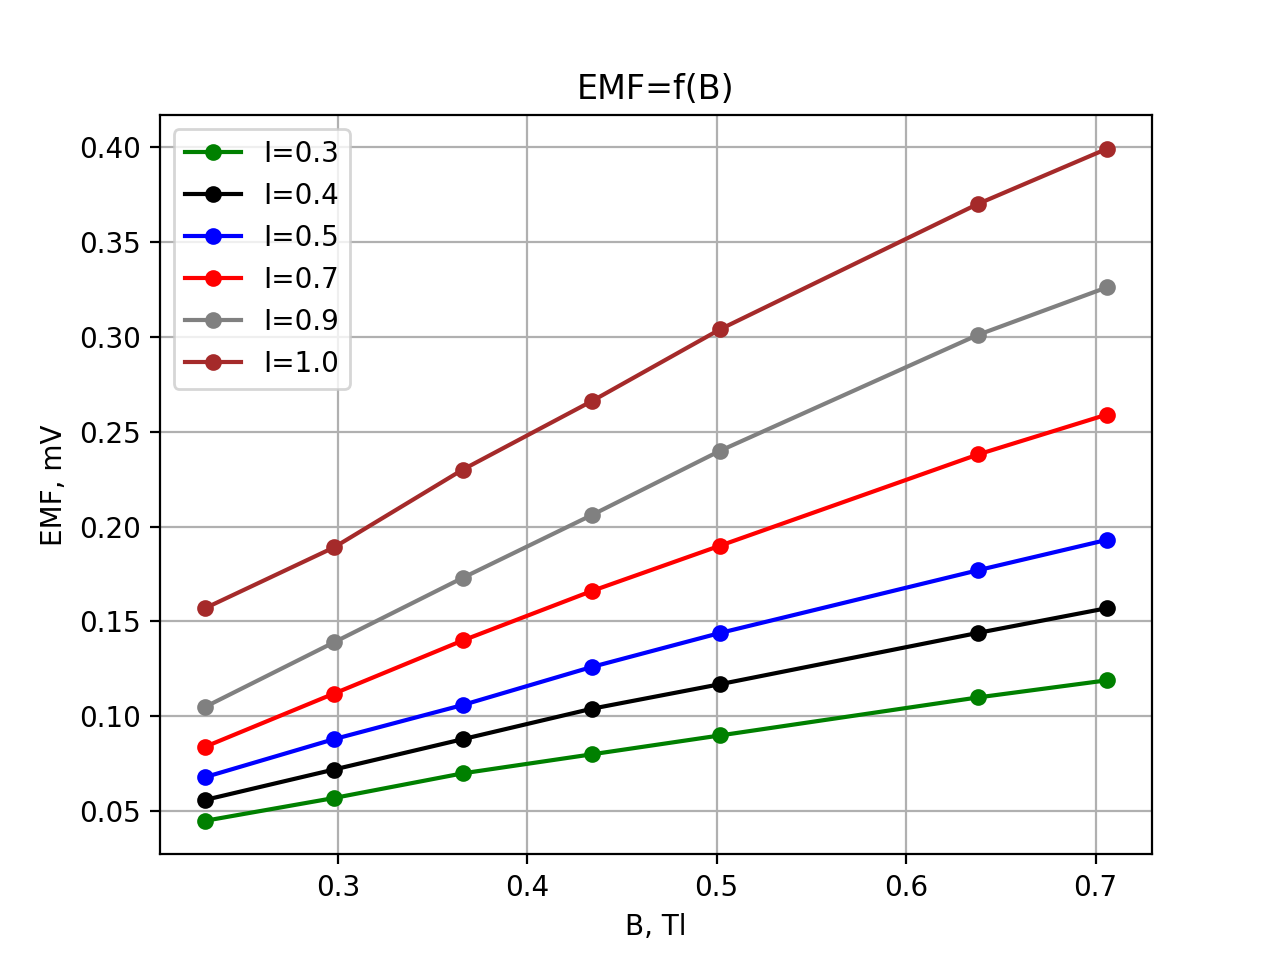
\includegraphics[width = 0.9 \textwidth]{emf}
			\caption{Построим по полученным данным график зависимости $\mathscr{E}_x = f(B)$ для разных $I$}
		\end{center}
	\end {figure}

\begin{table}[H]
	\centering
		\begin{tabular}{|c|c|c|c|c|c|c|c|}
			\hline
			$I_{34}, \text{ мА}$&	0,3	&0,4&	0,5	&	0,7	&0,9&	1 \\ \hline
			$k, \text{ мВ/Tл}	$&0,1544	&0,2112	&0,2623	&	0,3671&	0,4682&	0,5161 \\ \hline
		\end{tabular}
	\caption{Углы наклона графиков в зависимости от $I_{34}$}
\end{table}

	\begin {figure}[H]
		\begin{center}
		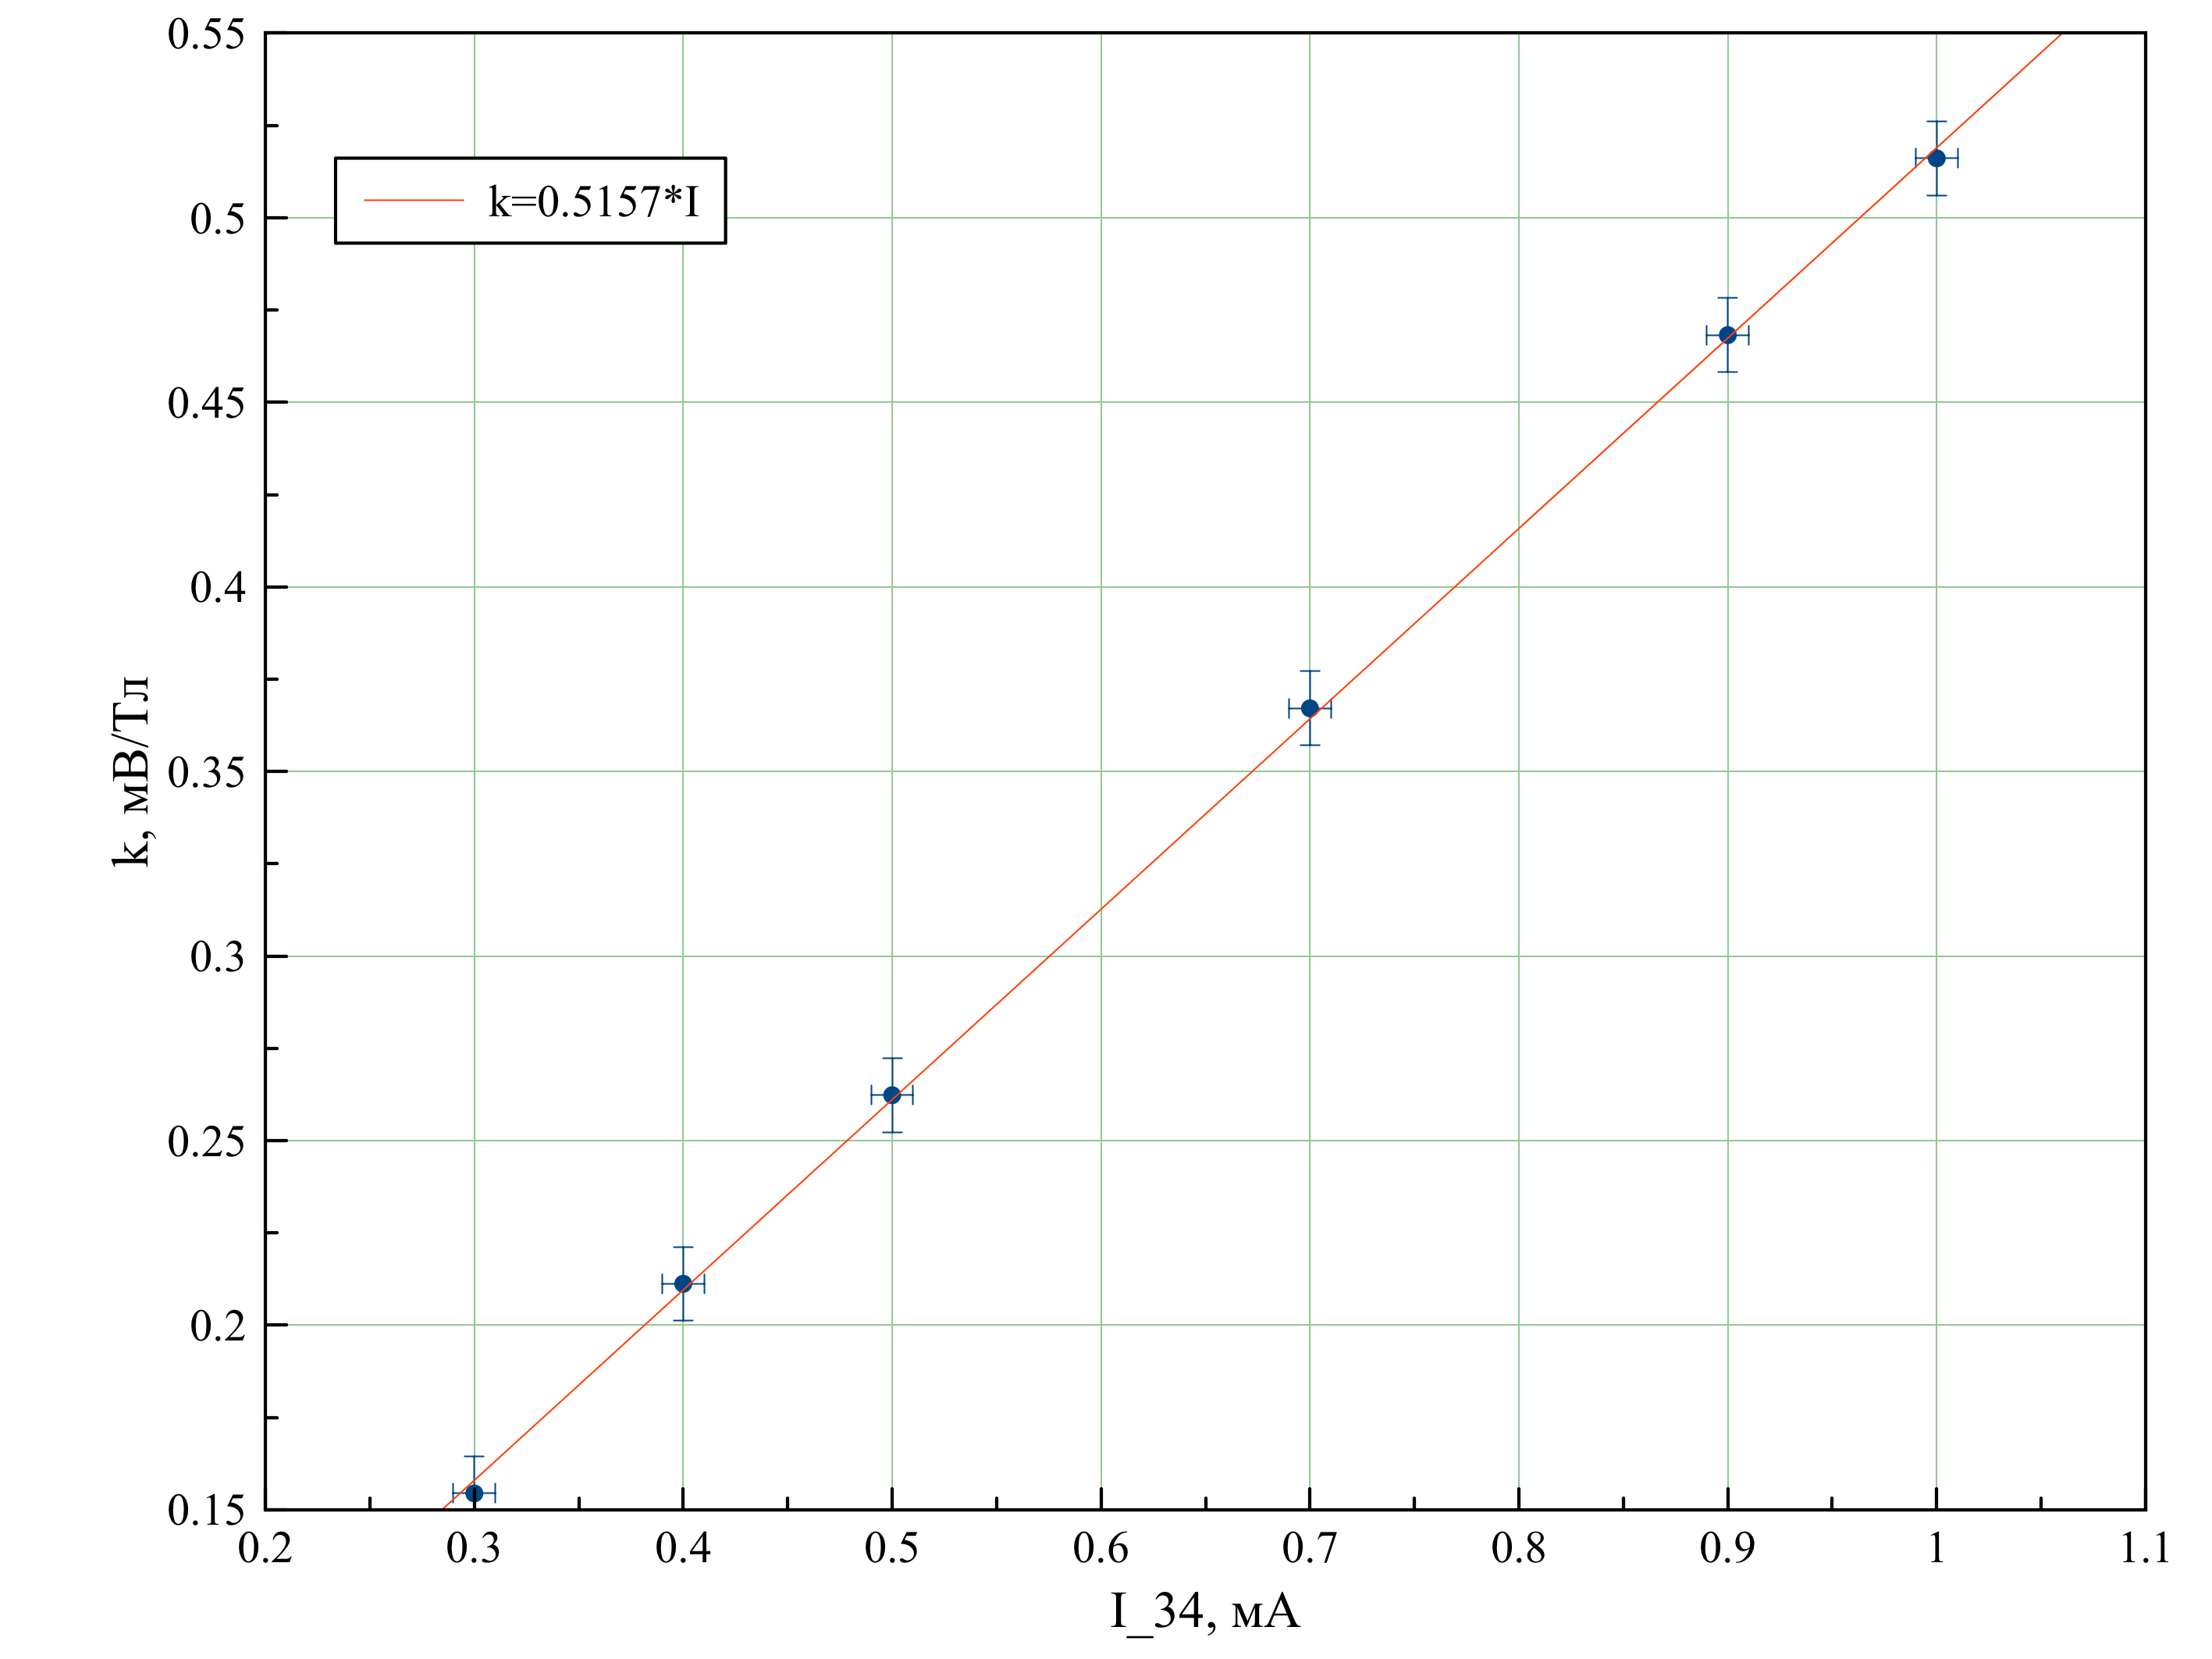
\includegraphics[width = 0.62 \textwidth]{angle}
			\caption{Построим по полученным углам наклона график зависимости $k = f(I)$}
		\end{center}
	\end {figure}


В итоге из графика получаем $$k_x = \cfrac{\mathscr{E}_x}{IB} = (515,7 \pm 10,0) \dfrac{\text{мкВ}}{\text{мА}\cdot \text{Тл}}$$

Клеммы 3 и 5, при токе $I=1 \text{ мА}$ получаем:
$$U_{35} = 1.68 \;\text{мВ}$$

Определим постоянную Холла: $$R_x = \dfrac{\mathscr{E}_x}{IB} \cdot a = k_x \cdot a = (77,4 \pm 1,5) \cdot 10^{-5}\; \text{м}^3/\text{Кл}$$

Определим концентрацию носителей заряда: $$n = \dfrac{1}{eR_x} = (80,7 \pm 1,6) \cdot 10^{20} \; 1/\text{м}^3$$
	
Вычислим удельную проводимость материала: 
$$\sigma = \dfrac{I L_{35}}{U_{35} al} = (700,3 \pm 8,4)~~ 1/(\text{Ом} \cdot \text{м})$$

Рассчитаем подвижность электронов:
$$b = \dfrac{\sigma}{en} = (5,4 \pm 0,1) \cdot 10^3 \dfrac{\text{см}^2}{\text{В} \cdot \text{с}}$$

\section{Вывод}

Убедились в теории возникновения дополнительного ЭДС Холла. Мы определили постоянную Холла для Германия. Полученная проводимость n-типа(характер -- электронный). Благодаря эффекту Холла смогли получить важнейшие параметры, определяющие состояние электронов в полупроводнике -- получили подвижность и концентрацию заряда в полупроводнике.

\end{document}
